\documentclass[a4paper, 11pt]{article}
\usepackage{ctex}
\usepackage[margin=1in]{geometry}
\usepackage{color}
\definecolor{myGray}{RGB}{31, 31, 31}
\usepackage{supertabular}
\usepackage[colorlinks,
            linkcolor=myGray,
            anchorcolor=blue,
            citecolor=green
            ]{hyperref}
\usepackage{listings}
\usepackage{bidi}
\usepackage{bidiftnxtra}


\title{PPCA2016大作业:带5级流水的MIPS模拟器}
\author{柯嵩宇}

\begin{document}
\maketitle
\tableofcontents

\newpage
\section{基本要求}
\subsection{时间}
	见课程主页
\subsection{实现语言}
	C++、Java等,不推荐使用Python,如果使用了其他的语言请提前告知助教以便助教配置评测环境
\subsection{代码管理与提交}
\subsubsection{Git}
	要求全程使用git作为版本管理工具,学习并正确使用git\footnote{正确使用:助教可以通过你们的历史版本和提交记录了解你们的工作情况。如果只有一次或者非常少量的提交记录,那么将被判定为不正确的使用Git,会在一定程度上影响成绩}。
\subsubsection{Bitbucket}
	要求把代码推送到bitbucket\footnote{一个与Github类似的远程代码仓库,区别在于Github在免费使用时创建私有仓库的权限,而bitbucket的每个账户可以有5个免费的私有仓库}上,在bitbucket上面的项目名字为\texttt{mips-simulator}\footnote{项目名字很重要,这个关系到评测,直接影响到助教能否正确的通过批量测试脚本获取你们的代码},并且给用户\texttt{BreakVoid}一个Read权限\footnote{禁止把仓库的权限设置成公开的(public)}。
\section{实现要求}
要求实现的是一个能够正确解释MIPS汇编语言中与整数运算有关的一个子集的模拟器。关于程序的正确性方面,要求实现的模拟器有和SPIM相同的行为。
\subsection{要求实现的汇编语言特性}
	一下提及的指令都以SPIM Quick Reference和SPIM的实际执行效果为准\footnote{SPIM Quick Reference: \url{http://acm.sjtu.edu.cn/compiler/spim_ref.html}}。
\subsubsection{汇编器指令}
	需要实现的MIPS汇编器指令如下:
	\begin{description}
		\item[.align n]
			Align the next datum on a $ 2^n $ byte boundary. For example, .align 2 aligns the next value on a word boundary. .align 0 turns off automatic alignment of .half, .word, .float, and .double directives until the next .data or .kdata directive.
		\item[.ascii str]
			Store the string in memory, but do not null-terminate it.
		\item[.asciiz str]
			Store the string in memory and null-terminate it.
		\item[.byte b1, ..., bn]
			Store the n values in successive bytes of memory.
		\item[.data]
			The following data items should be stored in the data segment. If the optional argument addr is present, the items are stored beginning at address addr.
		\item[.half h1, ..., hn]
			Store the n 16-bit quantities in successive memory halfwords.
		\item[.space n]
			Allocate n bytes of space in the current segment (which must be the data segment in SPIM).
		\item[.text]
			The next items are put in the user text segment. In SPIM, these items may only be instructions or words (see the .word directive below). If the optional argument addr is present, the items are stored beginning at address addr.
		\item[.word w1, ..	., wn]
Store the n 32-bit quantities in successive memory words.
	\end{description}
\subsubsection{SPIM指令集}
	算术和逻辑指令\footnote{下面提及的Rdest为存储结果的寄存器,Rsrc, Rsrc1, Rsrc2为操作数所在的寄存器,Src2表示这个操作数既可以是立即数也可以是一个寄存器中的数据(即寄存器标号)}:
	\begin{itemize}
		\item abs Rdest, Rsrc	\hfill Absolute Value
		\item add Rdest, Rsrc1, Src2	\hfill Addition (with overflow)
		\item addi Rdest, Rsrc1, Imm	\hfill Addition Immediate (with overflow)
		\item addu Rdest, Rsrc1, Src2	\hfill Addition (without overflow)
		\item addiu Rdest, Rsrc1, Imm	\hfill Addition Immediate (without overflow)
		\item and Rdest, Rsrc1, Src2	\hfill AND
		\item andi Rdest, Rsrc1, Imm	\hfill AND Immediate
		\item div Rdest, Rsrc1, Src2	\hfill Divide (with overflow)
		\item divu Rdest, Rsrc1, Src2	\hfill Divide (without overflow)
		\item mul Rdest, Rsrc1, Src2	\hfill Multiply (without overflow)
		\item mulo Rdest, Rsrc1, Src2	\hfill Multiply (with overflow)
		\item mulou Rdest, Rsrc1, Src2	\hfill Unsigned Multiply (with overflow)
		\item neg Rdest, Rsrc	\hfill Negate Value (with overflow)
		\item negu Rdest, Rsrc	\hfill Negate Value (without overflow)
		\item nor Rdest, Rsrc1, Src2	\hfill NOR
		\item not Rdest, Rsrc	\hfill NOT
		\item or Rdest, Rsrc1, Src2	\hfill OR
		\item ori Rdest, Rsrc1, Imm	OR \hfill Immediate
		\item rem Rdest, Rsrc1, Src2	\hfill Remainder\footnote{Put the remainder from dividing the integer in register Rsrc1 by the integer in Src2 into register Rdest. Note that if an operand is negative, the remainder is unspecified by the MIPS architecture and depends on the conventions of the machine on which SPIM is run.}\footnote{On my computer, \texttt{rem -5 2} and \texttt{rem -5 -2}  both return -1 which is same to C++'s remainder.}
		\item remu Rdest, Rsrc1, Src2	\hfill Unsigned Remainder
		\item rol Rdest, Rsrc1, Src2	\hfill Rotate Left\footnote{Rotate the contents of register Rsrc1 left (right) by the distance indicated by Src2 and put the result in register Rdest.}
		\item ror Rdest, Rsrc1, Src2	\hfill Rotate Right

		\item sll Rdest, Rsrc1, Src2	\hfill Shift Left Logical
		\item sllv Rdest, Rsrc1, Rsrc2	\hfill Shift Left Logical Variable
		\item sra Rdest, Rsrc1, Src2	\hfill Shift Right Arithmetic
		\item srav Rdest, Rsrc1, Rsrc2	\hfill Shift Right Arithmetic Variable
		\item srl Rdest, Rsrc1, Src2	\hfill Shift Right Logical
		\item srlv Rdest, Rsrc1, Rsrc2	\hfill Shift Right Logical Variable
		\item sub Rdest, Rsrc1, Src2	\hfill Subtract (with overflow)
		\item subu Rdest, Rsrc1, Src2	\hfill Subtract (without overflow)
		\item xor Rdest, Rsrc1, Src2	\hfill XOR
		\item xori Rdest, Rsrc1, Imm	\hfill XOR Immediate
	\end{itemize}
	常数操作指令:
	\begin{itemize}
		\item li Rdest, imm	\hfill Load Immediate
		\item lui Rdest, imm	\hfill Load Upper Immediate\footnote{Load the lower halfword of the immediate imm into the upper halfword of register Rdest. The lower bits of the register are set to 0.}
	\end{itemize}
	比较指令\footnote{对于所有的比较指令,结果为真返回1,结果为假则返回-1}:
	\begin{itemize}
		\item seq Rdest, Rsrc1, Src2	\hfill Set Equal\footnote{Set register Rdest to 1 if register Rsrc1 equals Src2 and to be 0 otherwise.}
		\item sge Rdest, Rsrc1, Src2	\hfill Set Greater Than Equal
		\item sgeu Rdest, Rsrc1, Src2	\hfill Set Greater Than Equal Unsigned
		\item sgt Rdest, Rsrc1, Src2	\hfill Set Greater Than
		\item sgtu Rdest, Rsrc1, Src2	\hfill Set Greater Than Unsigned
		\item sle Rdest, Rsrc1, Src2	\hfill Set Less Than Equal
		\item sleu Rdest, Rsrc1, Src2	\hfill Set Less Than Equal Unsigned
		\item slt Rdest, Rsrc1, Src2	\hfill Set Less Than
		\item slti Rdest, Rsrc1, Imm	\hfill Set Less Than Immediate
		\item sltu Rdest, Rsrc1, Src2	\hfill Set Less Than Unsigned
		\item sltiu Rdest, Rsrc1, Imm	\hfill Set Less Than Unsigned Immediate
		\item sne Rdest, Rsrc1, Src2	\hfill Set Not Equal
	\end{itemize}
	分支与跳转\footnote{每条MIPS的汇编指令都可以有一个或者多个label,分支与跳转语句中的label就是汇编指令的label,用于跳转到具有特定label的语句,注意label是全局唯一的}:
	\begin{itemize}
		\item b label	\hfill Branch instruction. \\
			Unconditionally branch to the instruction at the label.
		\item beq Rsrc1, Src2, label	\hfill Branch on Equal
		\item beqz Rsrc, label	Branch on Equal Zero
		\item bge Rsrc1, Src2, label	\hfill Branch on Greater Than Equal
		\item bgeu Rsrc1, Src2, label	\hfill Branch on GTE Unsigned
		\item bgez Rsrc, label	\hfill Branch on Greater Than Equal Zero
		\item bgezal Rsrc, label	\hfill Branch on Greater Than Equal Zero And Link
		\item bgt Rsrc1, Src2, label	\hfill Branch on Greater Than
		\item bgtu Rsrc1, Src2, label	\hfill Branch on Greater Than Unsigned
		\item bgtz Rsrc, label	\hfill Branch on Greater Than Zero
		\item ble Rsrc1, Src2, label	\hfill Branch on Less Than Equal
		\item bleu Rsrc1, Src2, label	\hfill Branch on Less Than Equal for Unsigned
		\item blez Rsrc, label	Branch on Less Than Equal Zero
		\item bgezal Rsrc, label	Branch on Greater Than Equal Zero And Link
		\item bltzal Rsrc, label	\hfill Branch on Less Than And Link
		\item blt Rsrc1, Src2, label	\hfill Branch on Less Than
		\item bltu Rsrc1, Src2, label	\hfill Branch on Less Than Unsigned
		\item bltz Rsrc, label	\hfill Branch on Less Than Zero
		\item bne Rsrc1, Src2, label	\hfill Branch on Not Equal
		\item bnez Rsrc, label	\hfill Branch on Not Equal Zero
		\item j label	\hfill Jump
		\item jal label	\hfill Jump and Link
		\item jalr Rsrc	\hfill Jump and Link Register \\
			Unconditionally jump to the instruction at the label or whose address is in register Rsrc. Save the address of the next instruction in register 31.
		\item jr Rsrc	\hfill Jump Register \\
			Unconditionally jump to the instruction whose address is in register Rsrc.
	\end{itemize}
	Load指令\footnote{从指定的内存地址读取数据并且保存到指定的寄存器,内存地址以\texttt{offset(Rhead)}或者是\texttt{label}的形式给出,即,寄存器中的首地址+偏移量,偏移量\textbf{可正可负}}:
	\begin{itemize}
		\item la Rdest, address	\hfill Load Address\footnote{Load computed address, not the contents of the location, into register Rdest.}
		\item lb Rdest, address	\hfill Load Byte
		\item lbu Rdest, address	\hfill Load Unsigned Byte \\
			Load the byte at address into register Rdest. The byte is sign-extended by the lb, but not the lbu, instruction.
		\item ld Rdest, address	\hfill Load Double-Word \\
			Load the 64-bit quantity at address into registers Rdest and Rdest + 1.
		\item lh Rdest, address	\hfill Load Halfword
		\item lhu Rdest, address	\hfill Load Unsigned Halfword \\
			Load the 16-bit quantity (halfword) at address into register Rdest. The halfword is sign-extended by the lh, but not the lhu, instruction
		\item lw Rdest, address	\hfill Load Word \\
		Load the 32-bit quantity (word) at address into register Rdest.
	\end{itemize}
	Store指令\footnote{从指定的内存地址读取数据并且保存到指定的寄存器,内存地址以\texttt{offset(Rhead)}或者是\texttt{label}的形式给出}:
	\begin{itemize}
		\item sb Rsrc, address	\hfill Store Byte \\
			Store the low byte from register Rsrc at address.
		\item sd Rsrc, address	\hfill Store Double-Word \\
			Store the 64-bit quantity in registers Rsrc and Rsrc + 1 at address.
		\item sh Rsrc, address	\hfill Store Halfword \\
			Store the low halfword from register Rsrc at address.
		\item sw Rsrc, address	\hfill Store Word \\
			Store the word from register Rsrc at address.
	\end{itemize}
	数据移动指令:
	\begin{itemize}
		\item move Rdest, Rsrc	\hfill Move \\
			Move the contents of Rsrc to Rdest.
	\end{itemize}
	特殊指令:
	\begin{itemize}
		\item nop	\hfill No operation \\
			Do nothing.\footnote{注意一下,这里的Do nothing并不是什么都不做,而是执行一条指令,指令的目的是什么都不做,它会在占用流水线并且按照5-stage的划分在每个阶段都占用相应的部分,这条指令主要是调试代码的时候使用。可以在每条语句执行之后插入nop指令,这样程序员就可以清楚的知道每一条指令的执行结果。}
		\item syscall \hfill System Call \\
			Register v0 contains the number of the system call (see System Services) provided by SPIM.\footnote{只需要模拟下面提到的几个系统调用即可}
	\end{itemize}
	系统调用:
	\begin{center}
		\begin{tabular}{|c|p{4cm}|p{4cm}|p{3cm}|}
			\hline
			系统调用编号 & 说明 & 参数 & 结果 \\
			\hline
			1 & 输出一个整数 & \$a0:需要输出的整数 & N/A \\
			\hline
			4 & 输出一个字符串,这个字符串要求以'\textbackslash 0'结尾 & \$a0:字符串的第一个字符的地址 & N/A \\
			\hline
			5 & 读入一个整数 & N/A & 读入的整数保存在\$v0 \\
			\hline
			8 & 读入一个字符串 & 
				\begin{tabular}{p{3.5cm}}
					\$a0:存放读入字符串的缓冲区 \\
					\$a1:读入最长的长度+1 \footnote{如果要读入'abc',那么\$a1应该设置成4或者更大} \\
				\end{tabular} & N/A \\
			\hline 
			9 & 分配堆内存 & \$a0:需要申请的连续的内存长度\footnote{单位:字节} & \$v0:申请结果,即内存片段的首地址\footnote{注意返回的地址要求首地址对齐到$ 2^2 $} \\
			\hline
			10 & 结束运行 & N/A & N/A \\
			\hline
			17 & 结束运行(有返回值)\footnote{C语言中的exit()函数} & \$a0:程序运行结束的返回值 & N/A \\
			\hline
		\end{tabular}
	\end{center}
\subsubsection{细节要求}
\subsubsection{5级流水划分}
	\begin{description}
		\item[Instruction Fetch] 取指令阶段,按照PC寄存器\footnote{表示当前执行到了那个内存地址的指令,这是一个特殊的寄存器,程序员无法直接修改这个寄存器的值}的值去指定的内存位置读取指令并且加载到寄存器中。
		\item[Instruction Decode \& Data Preparation] 对Instruction Fetch(IF)(取指令)阶段得到的指令进行解码,并且准备计算所需要的数据
		\item[Execution] 执行完成这个条指令必要的运算,对于算术和逻辑运算,那么计算出运算结果,对于内存操作,那么计算出实际需要load/store的内存地址\footnote{实际内存地址通过首地址+偏移量的形式给出,所以需要进行一次加法操作},对于分支指令,可以不用执行运算,但是实际上的MIPS的CPU是通过当前的PC寄存器的值+一个跳转指令的偏移量计算出最终的跳转位置。
		\item[Memory Access] 访问内存,完成load/store操作。
		\item[Write Back] 回写,把算术,或者逻辑运算的结果写到指定寄存器,把从内存中load到的数据写入指定的寄存器。对于分支语句,在这个阶段会改写PC寄存器。
	\end{description}
\subsubsection{寄存器读写顺序}
	由于流水线的存在,所以可能在同一个CPU时钟周期里面既要读寄存器又要写寄存器,先读还是先写会影响结果的正确性,所以我们规定,同一个CPU时钟周期里面先写寄存器,再读寄存器\footnote{如果把一个周期分成两个半周期,那么可以简单的认为,前半周期写,后半周期读}
\subsubsection{对于Hazard的处理}
	流水线在处理的过程中由于各种原因会导致流水线不能像期望的那样正常工作,下面有三大类Hazard\footnote{在CAAQA的中文版中,Hazard被翻译成冒险,但是几乎所有的人都认为这个翻译并不是那么合理,所以我在这里就直接使用英文而不是用中文翻译}:
	\begin{description}
		\item[Structure Hazard] 由于内存是总线上的设备,而总线的特性是同一时间\footnote{1个时钟周期}只能接受并执行一个任务请求,即不能再一个周期里面同时执行读取和写入(或者两个读取内存的操作)内存的操作,因此会造成流水线不能正常工作。举个例子,在每条指令的IF阶段都需要读取内存获取相应的内存,而第四个阶段Memory Access(MEM)中load/store指令也会读取或者写入内存,因此会造成总线的操作冲突,流水线因此停滞。
		\item[Data Hazard] 由于寄存器的内容只有当指令执行到第五个Write Back阶段才会更新,所以,对于数据有依赖的情况,流水线就不能正常的运转,需要等在前一个指令完全完成操作才行。
		\item[Control Hazard] 对于分支语句和跳转语句之后的语句不能轻易的上流水线,所以就会造成流水线停滞。
	\end{description}
	当Hazard发生的时候,模拟器应采取最暴力的做法,等待Hazard消失,然后重新启动流水线。
\section{MIPS汇编语言快速介绍}
\subsection{汇编语法}
	\begin{quotation}
		\texttt{(Label ':')$^*$ (Instruction | Directive) NEWLINE}
		\begin{description}
			\item [Label] 由字母(大小写敏感,数字和下划线以及其他一部分的可见符号\footnote{具体有哪些符号可以用并没有尝试过})构成的字符串,每一个Label后面有一个冒号,一个语句可以有一个或者多个Label\footnote{Label可以理解为指针,指向特定的内存地址}。
			\item [Instruction] MIPS汇编指令
			\item [Directive] 汇编器指令,用于分配静态内存空间,说明代码的存放位置。
			\item [NEWLINE] 换行符
		\end{description}
	\end{quotation}
\subsection{汇编语言执行细节}
	在正式执行汇编程序之前,汇编器会读取整个文件,按照文件的顺序理解每一个语句,如果这条语句是汇编器指令,那么就会按照要求执行相应的操作,例如分配一定长度的内存,对于出现在data区的Label,改Label指向的是这个Label后面一个data成员的内存地址。例如
	
	\begin{quotation}
\begin{lstlisting}[frame=single]
	.word 5
static_b:
	.word 10
\end{lstlisting}
	其中\texttt{static\_b}在内存中指向如图\ref{fig:static-b}。
	\end{quotation}
	\begin{figure}[htbp]
		\centering
		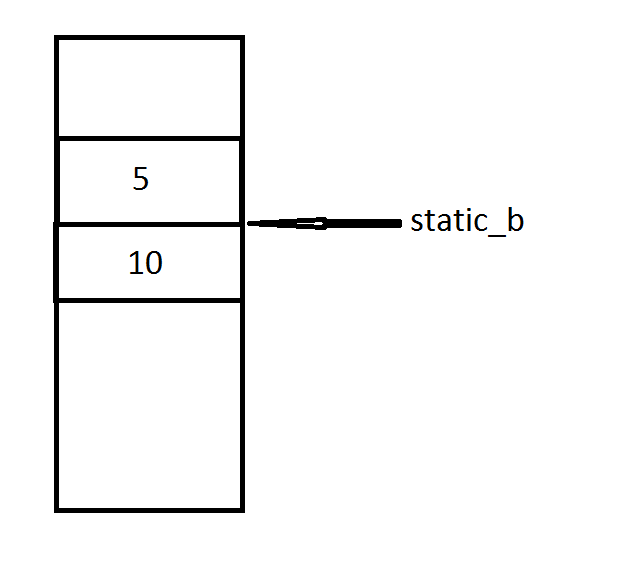
\includegraphics[width=0.5\textwidth]{label-to-data}
		\caption{static\_b指向的位置}
		\label{fig:static-b}
	\end{figure}
\subsection{内存细节}
	\begin{figure}[htbp]
		\centering
		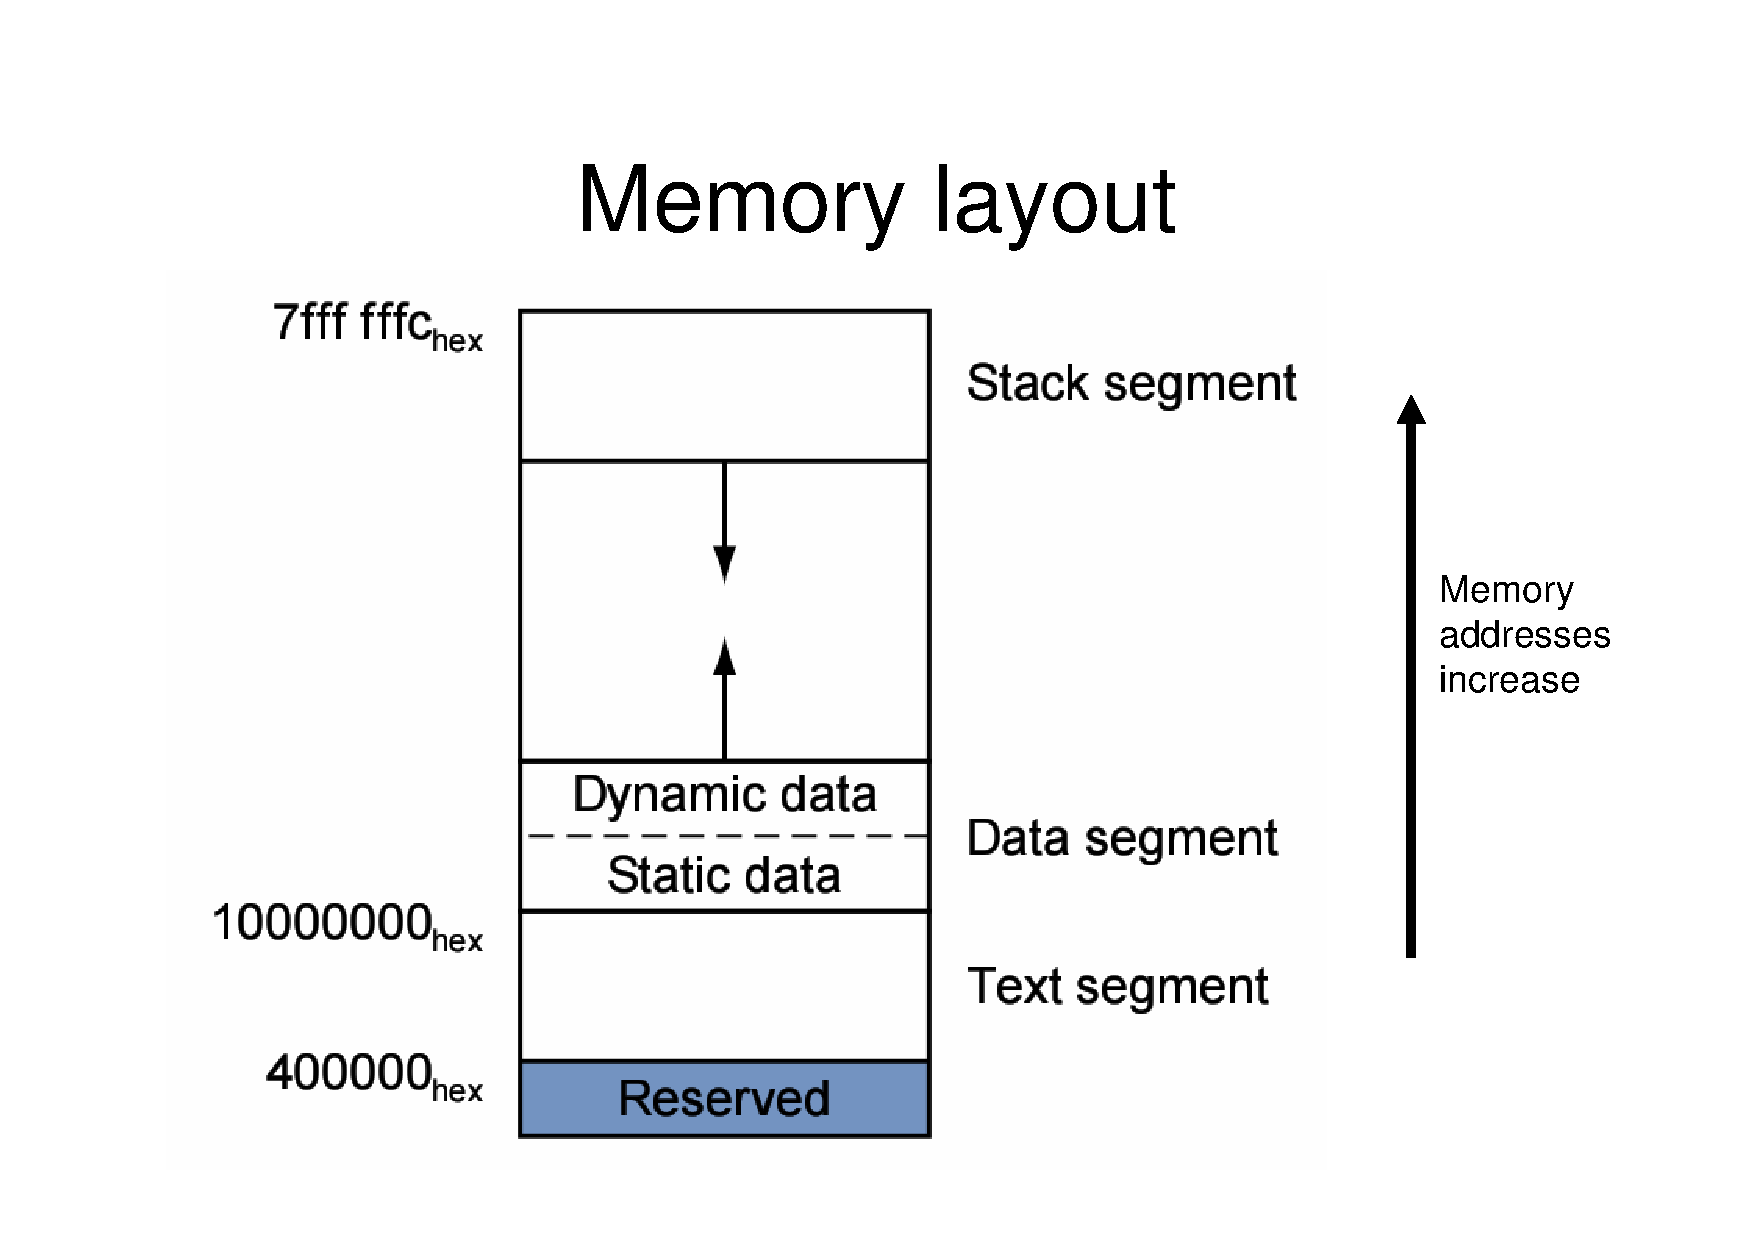
\includegraphics[angle=-90, width=0.7\textwidth]{SpimTutorial-page-7}
		\caption{内存分配}
		\label{fig:memory-alloc}
	\end{figure}
	MIPS的内存分配有一定顺序,栈空间从高地址开始到低地址,堆空间和静态空间从低地址开始到高地址,如图\ref{fig:memory-alloc},对于之前的那个例子,如果执行\texttt{lw \$t1, static\_b},则\texttt{\$t1}的值是10。
\subsection{寄存器的初始化}
	PC寄存器指向第一条指令,\$sp寄存器指向栈的最高地址(\texttt{0x80000000}),但是实际运行的时候由于运行时参数的原因\$sp会指向比\texttt{0x80000000}低的地址,具体情况可以参考QtSpim的Data区显示。\footnote{由于执行时的参数在测试数据中应该不会出现,所以可以简单的把\$sp寄存器的值定为\texttt{0x7ffffffc}}
\subsection{多字节load/store指令实现细节}
	对于单字节的lb和sb指令,模拟器精确地操作相应地址的内存区域,对于多字节的load和store指令做出如下约定:
	\begin{description}
		\item [对于lh和sh] 从addr+1读取最低的8位(0-7),从addr读取8位(8-15)\footnote{addr为传给指令的参数} 或把最低的8位写入到addr+1,把(8-15)写入到addr
		\item [对于lw和sw] 最低的8位对应addr+3,(8-15)对应addr+2,(16-23)对应addr+1,(24-31)对应addr。
	\end{description}
\subsection{其余细节}
	等待Q\&A之后补充
\end{document}
